\documentclass[11pt,letterpaper]{article}
\usepackage[utf8]{inputenc}
\usepackage[margin=1in]{geometry}
\usepackage{amsmath}
\usepackage{amsfonts}
\usepackage{amssymb}
\usepackage{amsthm}
\usepackage{verbatim}
\usepackage{graphicx}
\usepackage[hidelinks=true]{hyperref}
\usepackage[margin=1cm]{caption}
% No paragraph tabs
\setlength{\parindent}{0pt}

% Define commands that will be widely used.
\newcommand{\br}{\ \\}
\newcommand{\tab}{\hspace*{2em}}

\title{Calculating the Density Profile of the Sun Using a Polytrope}
\author{Rachel Domagalski}
\date{}

\begin{document}
\maketitle

\section{Introduction}

The density profile of a star can be modeled using a polytrope of an ideal gas.
This is just an approximation and a real star will not behave like that exactly.
The polytopic equation of state can be written as \cite{textbook}
\begin{equation}
    P = K \rho^\gamma = K \rho^{\frac{n+1}{n}}
    \label{polystate}
\end{equation}
where $P$ is the pressure of the gas, $\rho$ is the density, and where $\gamma$
is the ratio of specific heats for a gas. It is often customary to write
$\gamma$ in terms of a polytropic index $n$, where $\gamma = \frac{n+1}{n}$. The
equation for hydrostatic equilibrium can be combined with
\eqref{polystate} to get Poisson's equation
\begin{equation}
    \frac{K}{4\pi G}\left(\frac{n+1}{n}\right)\frac{1}{r^2}\frac{d}{dr}
    \left(\frac{r^2}{\rho^{\frac{n-1}{n}}}\frac{d\rho}{dr}\right) = -\rho
    \label{poisson_allconst}
\end{equation}
for $\rho\left(r\right)$ where $G$ is the gravitational constant. This equation
shall be solved using the center density of the sun as
$\rho\left(r = 0.007 R_{\bigodot} \right) = 150 \ g/cm^3$ and $\gamma = 5/3$.
This value of $\gamma$ gives a polytropic index of $n = 3/2$.

\section{Simplifying Poisson's equation}

In order to simplify the notation of Poisson's equation, the constant $\beta$
shall be defined as
\begin{equation}
    \beta^2 \equiv \frac{K}{4\pi G}\left(\frac{n+1}{n}\right) = 
    \frac{K \gamma}{4\pi G}
    \label{betadef}
\end{equation}

The textbook defines a constant $\alpha$ when deriving the Lane-Emden equation,
which is different from \eqref{betadef}. The constant $\beta$ is much more
convenient to work with than $\alpha$, given the form of
\eqref{poisson_allconst}. A simple relation between $\beta$ and $\beta$ will be
derived later. Poisson's equation \eqref{poisson_allconst} can now be written as
\begin{equation}
    \frac{\beta^2}{r^2}\frac{d}{dr}
    \left(\frac{r^2}{\rho^{\frac{n-1}{n}}}\frac{d\rho}{dr}\right) = -\rho
    \label{poisson_eq}
\end{equation}

The strategy now is to reduce \eqref{poisson_eq} from a second order
differential equation to a system of first order equations. In order to do this,
a function $u\left(r\right)$ shall be defined as
\begin{equation}
    u \equiv \frac{d\rho}{dr}
\end{equation}

Multiplying \eqref{poisson_eq} by $r^2 / \beta^2$ gives
\begin{equation}
    \frac{d}{dr}\left(r^2\rho^\frac{1-n}{n}u\right) = -\frac{r^2}{\beta^2}\rho
    \label{derivative}
\end{equation}

The left hand side of \eqref{derivative} can be expanded as
\begin{equation}
    \frac{d}{dr}\left(r^2\rho^\frac{1-n}{n}u\right) =
    2r \rho^\frac{1-n}{n}u + r^2 \rho^\frac{1-n}{n} \frac{du}{dr} +
    r^2 \left(\frac{1-n}{n}\right) \rho^\frac{1-2n}{n} u^2
    = -\frac{r^2}{\beta^2}\rho
    \label{almostthere}
\end{equation}

The $\frac{du}{dr}$ term can be isolated by multiplying \eqref{almostthere} by
$\rho^\frac{n-1}{n}$ and dividing by $r^2$.
\begin{equation}
    \frac{2u}{r} + \frac{du}{dr} + \left(\frac{1-n}{n}\right)\frac{u^2}{\rho}
    = -\frac{1}{\beta^2} \rho^\frac{2n-1}{n}
\end{equation}

The original second order differential equation \eqref{poisson_eq} can now be
expressed as a system of two first order equations with $u$ and $\rho$ as the
dependent variables.

\begin{equation}
    \begin{array}{rcl}
        \dfrac{d\rho}{dr} & = & u\\
        \ \\
        \dfrac{du}{dr} & = & \left(\dfrac{n-1}{n}\right)\dfrac{u^2}{\rho}
        -\dfrac{2u}{r} -\dfrac{1}{\beta^2} \rho^\frac{2n-1}{n} \\
    \end{array}
    \label{exactsystem}
\end{equation}

It should be noted that the system described in \eqref{exactsystem} is singular
when $r = 0$ or $\rho = 0$. This shouldn't be surprising as this can be deduced
from \eqref{poisson_eq}. Fortunately, the initial condition given for this
problem is not at the singular point, despite being nearby. It is worth
mentioning that in order to solve this equation, both initial conditions for the
density and density gradient are needed. While the center density gradient is
not given, its value can and will be argued to be zero.

\section{Creating a numerical scheme}

The system of first order equations in \eqref{exactsystem} can be made into a
scheme for a numerical solution. An easy way to represent derivatives is to
make the following approximation
\begin{displaymath}
    \frac{dy}{dx} = \frac{y_{i+1} - y_i}{h}
\end{displaymath}
where $h$ is the step size between each $x_i$. The system described in
\eqref{exactsystem} can now be represented as difference equations.

\begin{equation}
    \begin{array}{rcl}
        \dfrac{\rho_{i+1} - \rho_i}{h} & = & u_i\\
        \ \\
        \dfrac{u_{i+1} - u_i}{h} & = &
        \left(\dfrac{n-1}{n}\right)\dfrac{u_i^2}{\rho_i}
        -\dfrac{2 u_i}{r_i} -\dfrac{1}{\beta^2} \rho_i^\frac{2n-1}{n} \\
    \end{array}
    \label{difference_eq}
\end{equation}

These difference equations can be written as iterations for step $i+1$.

% Euler method iteration method.
\begin{equation}
    \begin{array}{rcl}
        \rho_{i+1} & = & \rho_i + h u_i\\
        \ \\
        u_{i+1} & = &
        u_i + h\left[\left(\dfrac{n-1}{n}\right)\dfrac{u_i^2}{\rho_i}
        -\dfrac{2 u_i}{r_i} -\dfrac{1}{\beta^2} \rho_i^\frac{2n-1}{n}\right]\\
    \end{array}
    \label{iteration_eq}
\end{equation}

The algorithm for solving the original second order equation is now clear.
First, the density of step $i+1$ can be calculated from the density and density
gradient of the $i^{th}$ step. After that, the density gradient of step $i+1$
must be calculated to get the next value of density. This repeats for the entire
radial range of interest of the differential equation.\\

The iteration scheme \eqref{iteration_eq} uses a method similar to Euler's
method to calculate the density and density gradient. In order to improve the
accuracy of the algorithm, a method similar to the Runge-Kutta method can be
developed. For notation convenience, \eqref{exactsystem} can be expressed as
functions $f^j\left(r, \rho, u\right)$.

% Rewrite functions on more compact / general notation
\begin{equation}
    \begin{array}{rcccl}
        \dfrac{d\rho}{dr} & = & f^1\left(r, \rho, u \right) & = & u\\
        \ \\
        \dfrac{du}{dr} & = & f^2\left(r, \rho, u\right) & = &
        \left(\dfrac{n-1}{n}\right)\dfrac{u^2}{\rho}
        -\dfrac{2u}{r} -\dfrac{1}{\beta^2} \rho^\frac{2n-1}{n} \\
    \end{array}
\end{equation}

A method of iteration similar to the classic fourth-order Runge Kutta method can
be compactly expressed using this notation
% RK4 scheme
\begin{equation}
    x^j_{i+1} =
    x^j_i + \frac{h}{6} \left(k^j_1 + 2k^j_2 + 2k^j_3 + k^j_4\right),
    \ j = 1,2
    \label{rungekutta4}
\end{equation}
where $j=1$ corresponds to $\rho$, $j=2$ corresponds to $u$, and where
\begin{equation} % Runge-Kutta coefficients
    \begin{array}{rcl}
        k^j_1 & = & 
            f^j\left(
                r_i,
                \rho_i,
                u_i
            \right) \\
        \ \\ % Add some line breaks.
        k^j_2 & = &
            f^j\left(
                r_i    + \dfrac{h}{2},
                \rho_i + \dfrac{h}{2} k^\rho_1,
                u_i    + \dfrac{h}{2} k^u_1
            \right) \\
        \ \\
        k^j_3 & = &
            f^j\left(
                r_i    + \dfrac{h}{2},
                \rho_i + \dfrac{h}{2} k^\rho_2,
                u_i    + \dfrac{h}{2} k^u_2
            \right) \\
        \ \\
        k^j_3 & = &
            f^j\left(
                r_i    + h,
                \rho_i + h k^\rho_3,
                u_i    + h k^u_3
            \right) \\
    \end{array}
    \label{rk4coefs}
\end{equation}

It should be noted that \eqref{poisson_eq} can be solved analytically for $n=1$
and $n=5$ and these solutions will be used as a check that the numerical scheme
is working properly. For $n = 3/2$, the system of differential equations can be
written as
\begin{equation}
    \begin{array}{rcl}
        \dfrac{d\rho}{dr} & = & u\\
        \ \\
        \dfrac{du}{dr} & = & \dfrac{u^2}{3\rho}
        -\dfrac{2u}{r} -\dfrac{1}{\beta^2} \rho^\frac{4}{3} \\
    \end{array}
    \label{poly32}
\end{equation}

\section{Initial conditions}

The value of $\rho_c$ used as an initial condition for the Poisson's equation is
$150\ g/cm^3$ \cite{textbook}. However, this is not for $r = 0$, but for
$r = 0.007 R_{\bigodot}$ since Poisson's equation is singular at $r = 0$. This
can be used to fix the constant $K$ from the polytropic equation of state, which
gives $K = P_c \rho_c^{-\gamma}$. The value for $P_c$ is
$P_c = 10^{17.369}\ dyn/cm^2$ \cite{textbook}, which gives $K$ a value of
$552.3 \times 10^{13}\ \frac{dyn\ cm^3}{g^{5/3}}$. This value of $K$ can be used
to calculate $\beta = 1.048 \times 10^{10}\ cm^{1/2} g^{1/6}$.
The units on $\beta$ may be odd, but $\beta$ depends on $K$, which has
dimensions that depend on $\gamma = 5/3$.\\

The initial condition for $\rho_c$ is not enough to solve Poisson's equation.
Additionally, an initial condition for $\frac{d\rho}{dr}$ at the center of the
star is needed. The density gradient can be argued to be zero at the center of
the star. This can be seen from the polytropic equation of state and from the
equation of hydrostatic equilibrium. The pressure gradient of a polytrope in
hydrostatic equilibrium is
\begin{equation}
    \frac{dP}{dr} =
    -\rho\left(r\right)\frac{GM\left(r\right)}{r^2} = 
    K\gamma \rho\left(r\right)^{\gamma-1} \frac{d\rho}{dr} 
\end{equation}
which implies that 
\begin{equation}
    \frac{d\rho}{dr} = -\frac{G\rho^{2-\gamma}M\left(r\right)}{K\gamma r^2}
\end{equation}

The mass $M\left(r\right)$ is at least of order $O\left(r^3\right)$ since
$dM = 4\pi r^2 \rho dr$, which means that
$\frac{M\left(r\right)}{r^2} \varpropto O\left(r\right)$. Therefore, it is clear
that when taken in the limit of $r \rightarrow 0$, $d\rho/dr$ goes to zero. It
can also be intuitively argued that the center of the sun is the region of
highest pressure, and this corresponds to a maximum in density, because of the
polytropic equation of state. This sets the initial condition on $d\rho/dr$
since the derivative of a function at a maximum is always zero. It can now be
said that all of the necessary initial conditions required to run the numerical
solution of Poisson's equation are available. 

\section{Checking the numerical scheme}

When using a certain class of solutions, Poisson's equation can be rewritten as
the Lane-Emden equation. This is done by using solutions of the form
$\rho\left(r\right) = \rho_c \theta^n\left(r\right)$. The Lane-Emden equation is
\cite{textbook}
\begin{equation}
    \frac{1}{\xi^2} \frac{d}{d\xi}
    \left(\xi^2\frac{d\theta\left(\xi\right)}{d\xi}\right) =
    -\theta^n\left(\xi\right)
\end{equation}
where $\xi = \dfrac{r}{\alpha}$ and
$\alpha^2 = \dfrac{P_c\left(n+1\right)}{4 \pi G \rho_c^2}$. The Lane-Emden
equation has analytical solutions for $n = 1$ and $n = 5$. It also has an
analytical solution for $n=0$, but since that doesn't correspond to a finite
value of $\gamma$, that solution will be ignored. The known analytical
solutions, which can be used to check the numerical scheme, are \cite{textbook}
\begin{equation}
    \begin{array}{rcl}
        \theta_1\left(\xi\right) & = & \dfrac{\sin\xi}{\xi} \\
        \ \\ 
        \theta_5\left(\xi\right) & = & \dfrac{1}{\sqrt{1 + \xi^2/3}} \\
    \end{array}
    \label{exact_theta}
\end{equation}

These analytical solution can be written in terms of $r$ and $\beta$, which can
be related to the initial conditions of the original problem. This can be done
by noting that
\begin{equation}
    \frac{\alpha^2}{\beta^2} =
    \frac{n P_c}{K \rho_c^2} =
    n \rho_c^{\frac{1-n}{n}}
\end{equation}
and using the definition $\rho\left(r\right) = \rho_c \theta^n\left(r\right)$ to 
show that
\begin{equation}
    \begin{array}{rcl}
        \rho_1\left(r\right) & = &
            \dfrac{\rho_c \beta}{r} \sin\left(r/\beta\right) \\ 
        \ \\
        \rho_5\left(r\right) & = &
            \rho_c\left(1 + \dfrac{\rho_c^{4/5}r^2}{15\beta^2}\right)^{-5/2}
    \end{array}
    \label{rho5}
\end{equation}

Plots illustrating tests of the numerical scheme can be seen in
Figure~\ref{exact_sols}. In both cases, 100 steps between $r = 0.007
R_{\bigodot}$ and $r = R_{\bigodot}$ were used to construct the numerical
solution and the numerical solution scheme used to create these calibration
plots was the $4^{th}$ order Runge-Kutta method described above. The first thing
to note is that in both cases where exact solutions to Poisson's equation exist,
the numerical solution and the exact solution are practically indistinguishable
from one another. This is a pretty good indicator that the numerical solver is
working correctly. It can also be seen from Figure~\ref{exact_sols} that the
relative error on the solutions is small and that there is no oscillatory
behavior in the error. This is a more quantitative measure that the numerical
scheme is working properly and that the results for solutions to Poisson's
equation that lack analytic solutions can be sufficiently trusted.

% Figures showing the exact solutions for n = 1
\begin{figure}
    \centering
    \begin{minipage}[t]{0.496\textwidth}
        \centering
        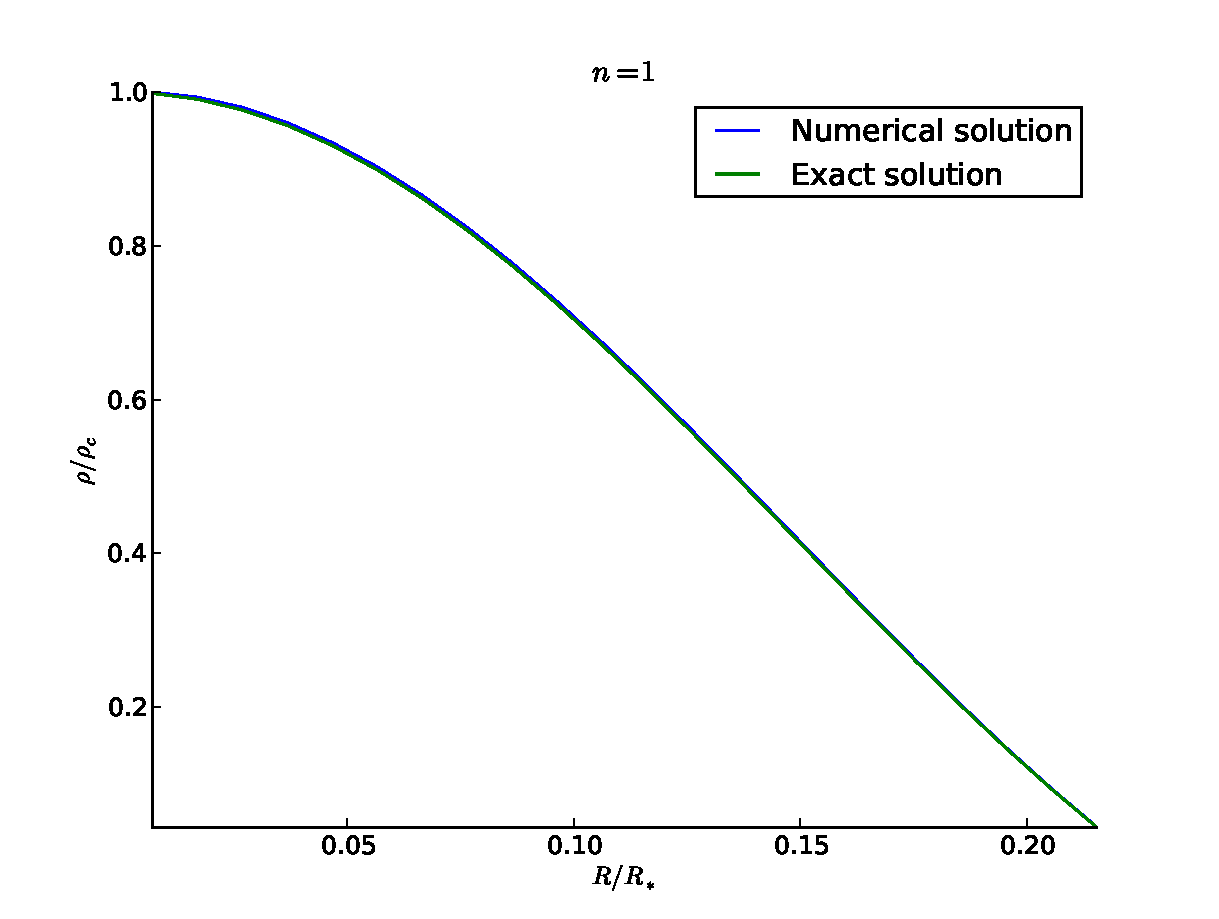
\includegraphics[width=\textwidth]{figures/poly1.pdf}
    \end{minipage}
    \begin{minipage}[t]{0.496\textwidth}
        \centering
        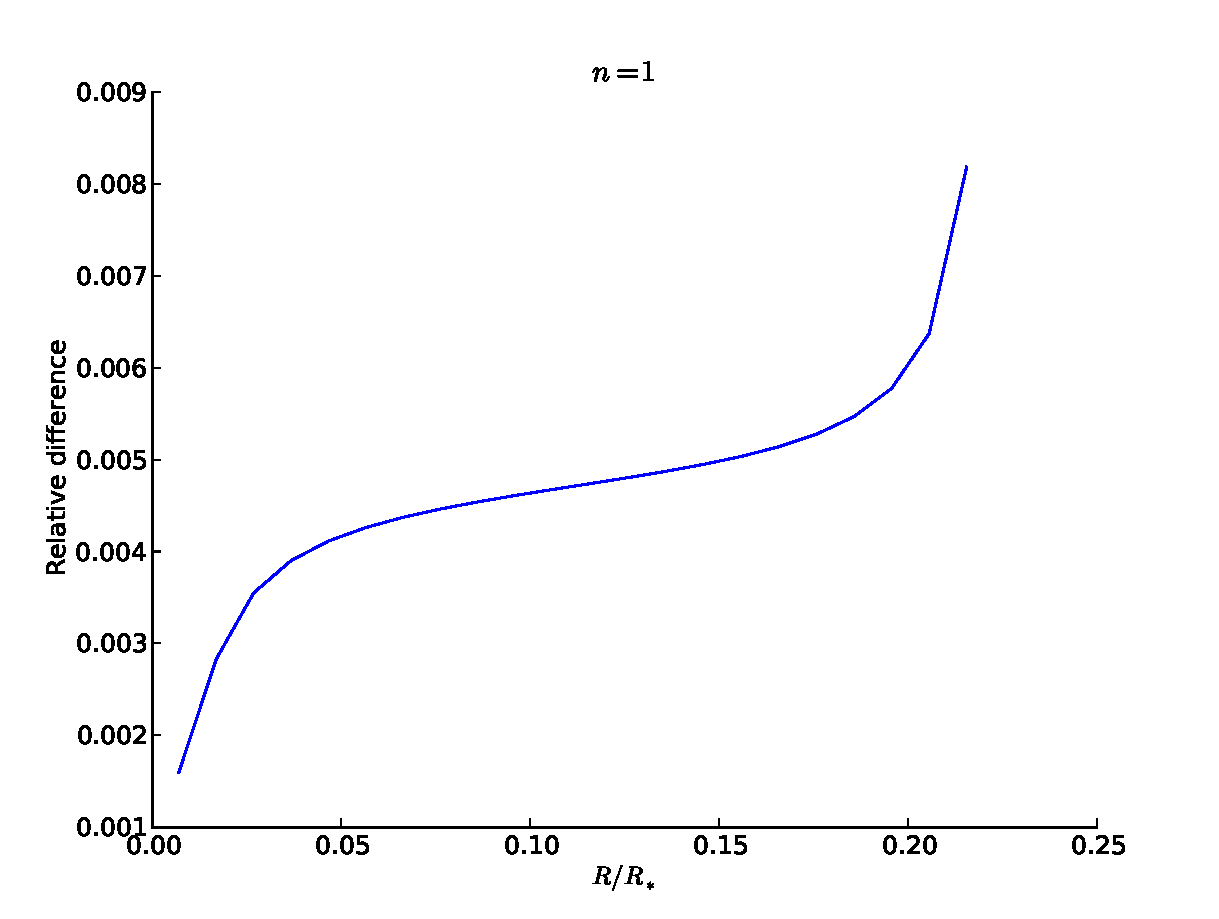
\includegraphics[width=\textwidth]{figures/poly1_err.pdf}
    \end{minipage}
    \begin{minipage}[t]{0.496\textwidth}
        \centering
        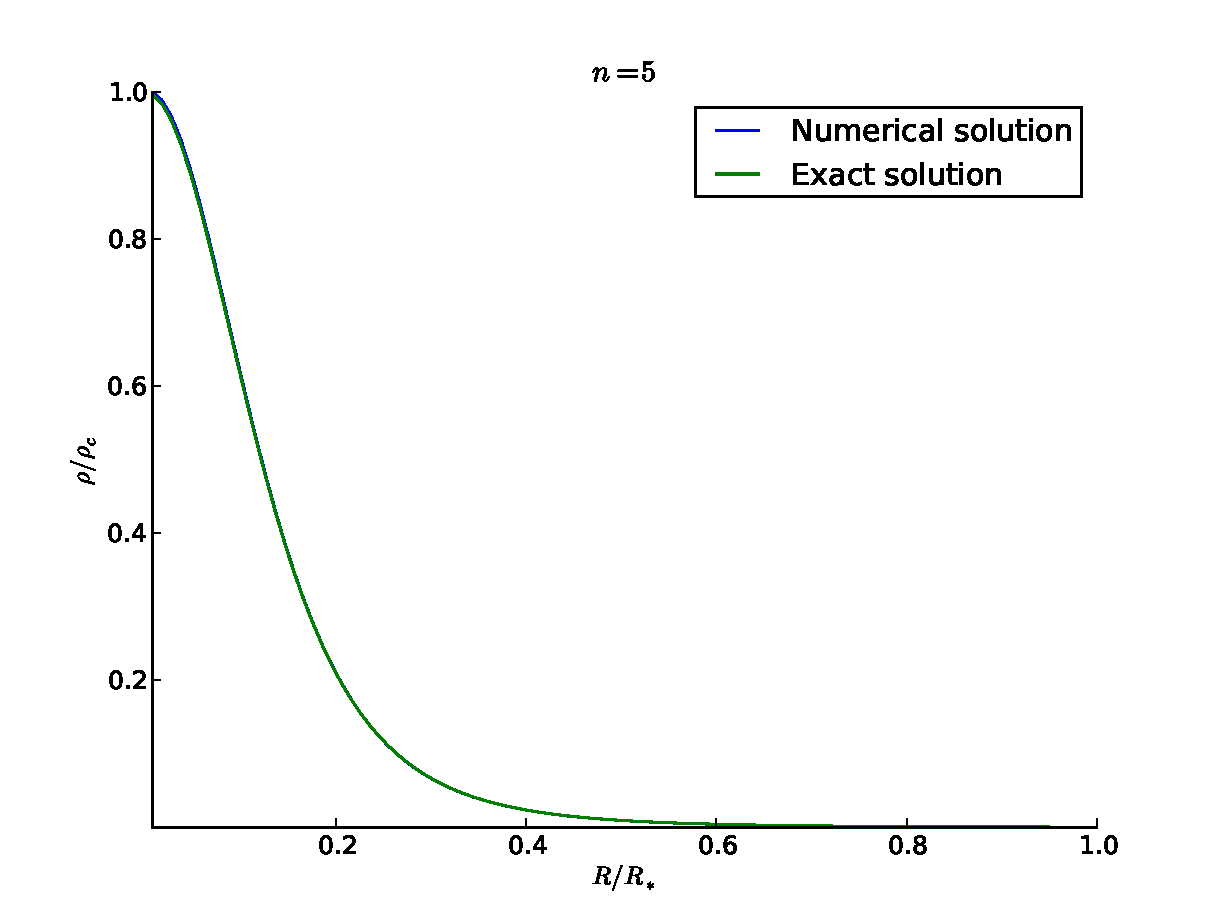
\includegraphics[width=\textwidth]{figures/poly5.pdf}
    \end{minipage}
    \begin{minipage}[t]{0.496\textwidth}
        \centering
        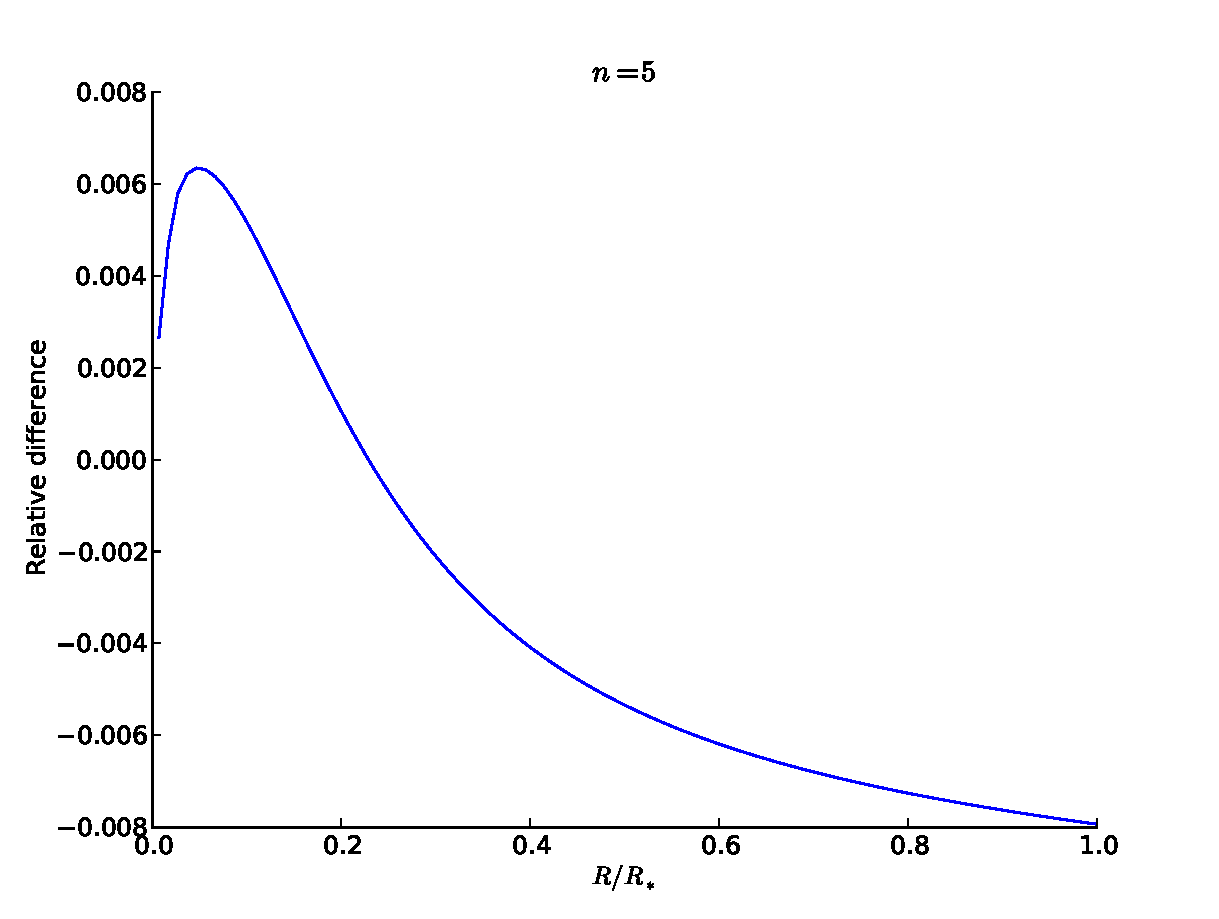
\includegraphics[width=\textwidth]{figures/poly5_err.pdf}
    \end{minipage}
    \caption{This figure is a test to verify that the solution algorithm is
    giving accurate results. The figures on the left are overlays of the
    numerical solutions with the exact solutions. The figures on the right are
    the errors of the numerical solution relative to the exact solution.}
    \label{exact_sols}
\end{figure}

\section{Results}

A numerical solution to a star with $\gamma = 5/3\ \left(n = 3/2\right)$ can be
seen in Figure~\ref{poly15} and a comparison of solutions for different
polytropic indexes can be seen in Figure~\ref{many_sols}.
The first thing to note is that the $n = 3/2$ solution only extends to about
$0.29 R_{\bigodot}$. Additionally, the solution for $n = 1$ only extends to
approximately $0.22 R_{\bigodot}$. This is because the solver was programmed to
stop when density goes negative. The reason for this is because negative density
does not make any physical sense. It should be noted that one cannot expect
solutions to be always positive for all radii. This can be seen from
\eqref{exact_theta}, where the analytic solution for $n = 1$ is a sinusoid. It
is possible that given the solar initial conditions, numerical solutions to
Poisson's equation will go negative before reaching $R_{\bigodot}.$\\

Since the solutions for $n = 1$ and $n = 3/2$ do not extend to $R_{\bigodot}$,
they are not good approximations for the sun, given its radius. An approximation
that represents the sun better can be seen in Figure~\ref{poly5data}, where
$n = 5$, which corresponds to $\gamma = 6/5$. In Figure~\ref{poly5data}, the
numerical solution for $n = 5$ is plotted against theoretical solar data found
in the textbook \cite{textbook}, and the numerical model seems decently match
the data given.\\

Source code for my solution can be found here:\\
\url{https://github.com/isaacdomagalski/astro160-polytrope}

\begin{figure}
    \centering
    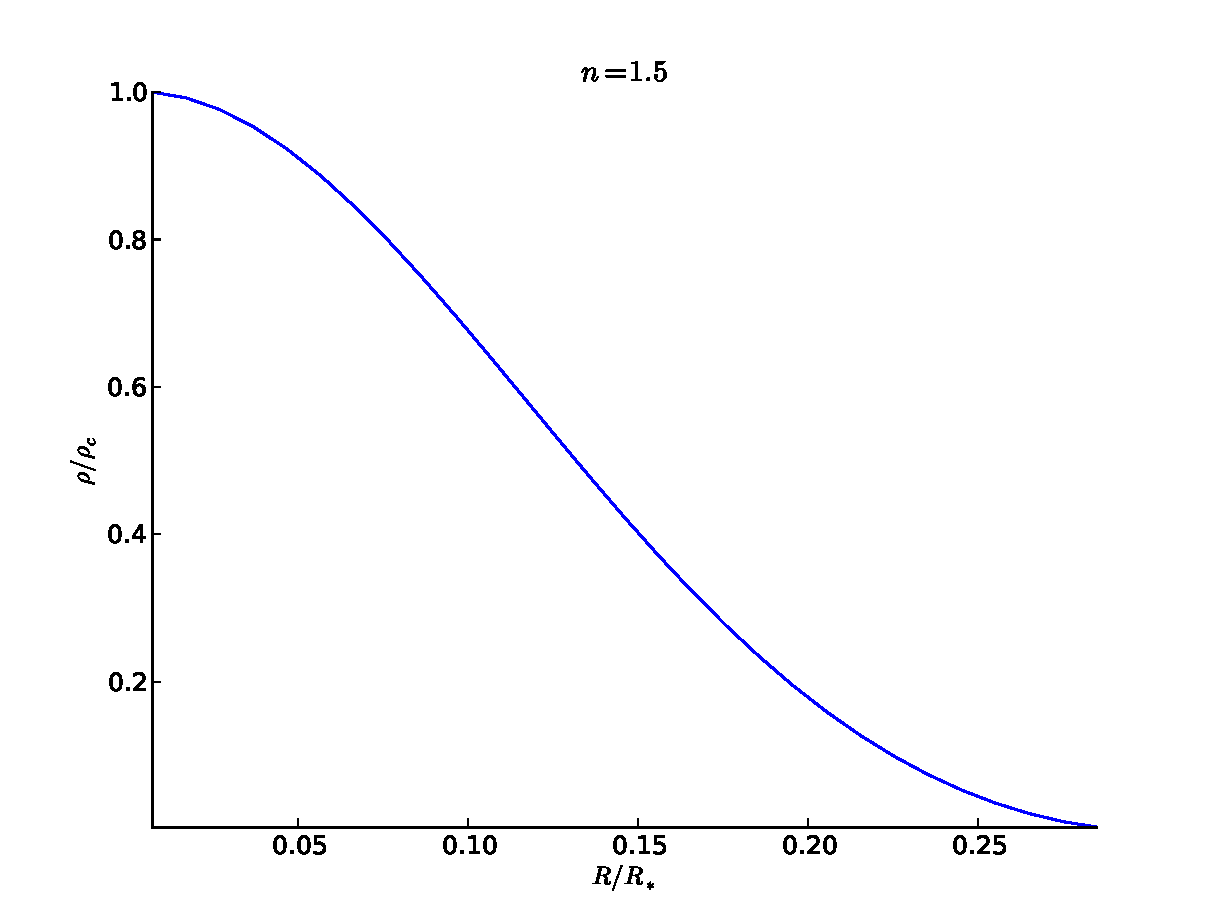
\includegraphics[width=0.75\textwidth]{figures/poly1_5.pdf}
    \caption{Numerical solution for a star with a polytropic index of $n=3/2$.}
    \label{poly15}
\end{figure}

\begin{figure}
    \centering
    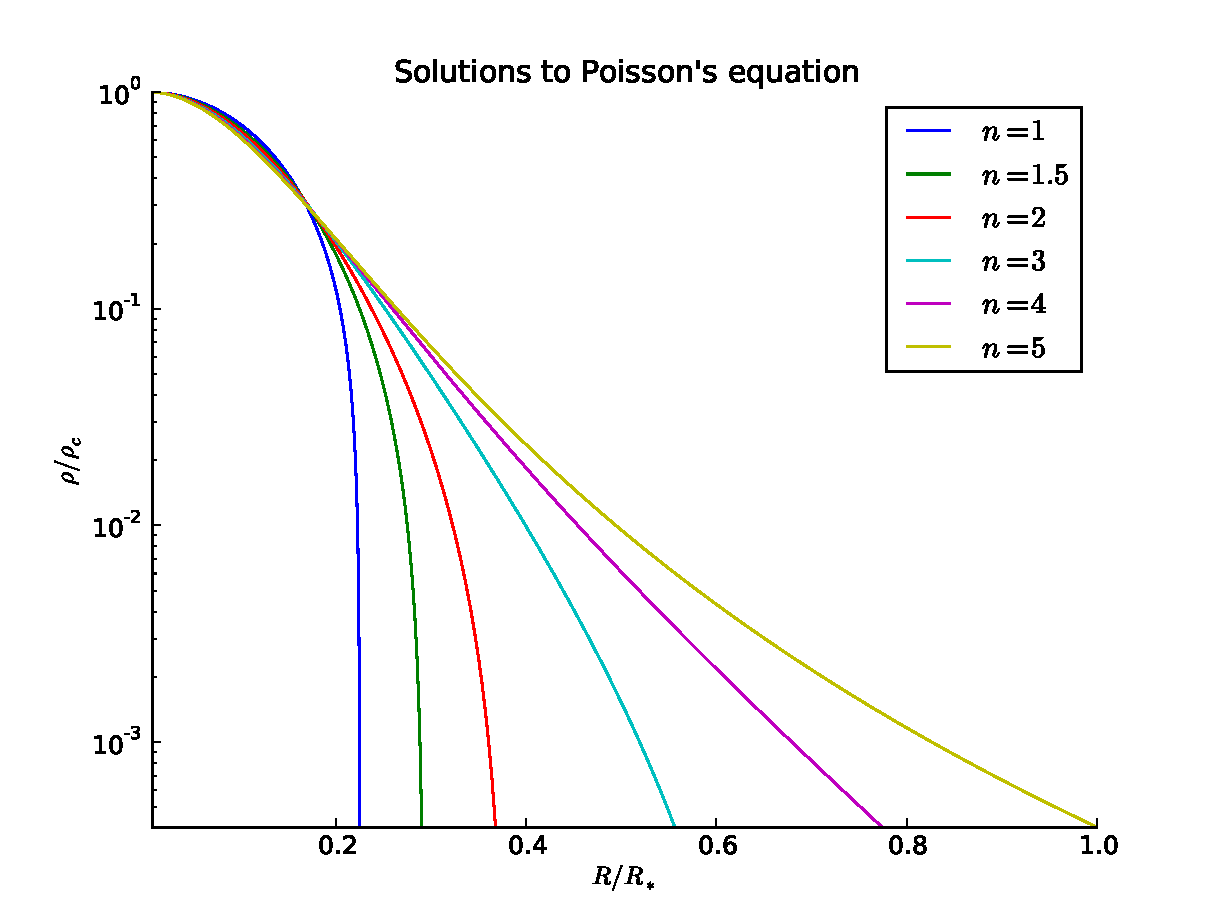
\includegraphics[width=0.75\textwidth]{figures/many_sols.pdf}
    \caption{This plot has solutions for multiple polytropic indexes. It should
    be noted that the x-axis is not at $\rho/\rho_c = 0$, but some small power
    of 10. Also, the step size between each iteration on this plot is
    $R_{\bigodot} / 10000$.}
    \label{many_sols}
\end{figure}

\begin{figure}
    \centering
    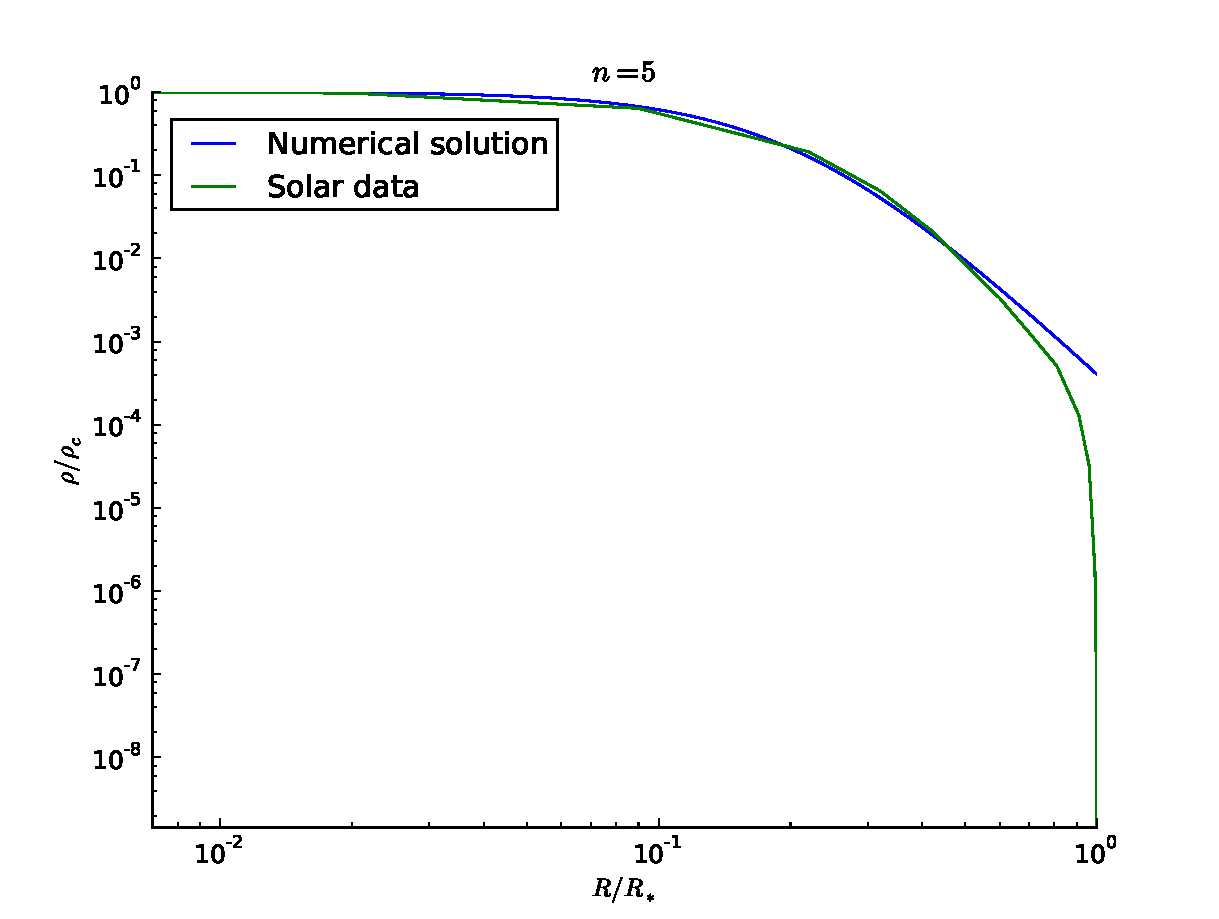
\includegraphics[width=0.75\textwidth]{figures/poly5_solar.pdf}
    \caption{Comparison of a polytropic star with $n=5$ and with theoretical
    solar data. This plot is a recreation of Figure~5.8 from the textbook.}
    \label{poly5data}
\end{figure}

\bibliographystyle{unsrt}
\bibliography{reference_list}{}

\end{document}  
